%! Author = chaorn
%! Date = 06.01.23
\subsubsection{JNDI Architektur und Funktionsweise}

Um das zugrunde liegende Problem besser verstehen zu können hilft ein etwas tieferer Einblick in die Architektur
und der grundlegenden Funktionalität der \gls{jndi} Bibliothek.
\begin{figure}[!htb] % ! - override default, h - place here, t - place figure at top of a page, b - place figure at bottom of a page
    \begin{center}
        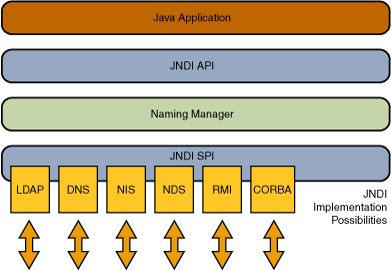
\includegraphics[scale=0.75]{images/jndiarch}
    \end{center}
    \caption{JNDI Architektur}
\end{figure}
\\
Das \gls{jndi} besteht im Grunde aus einer \gls{api} und einem \gls{spi}. Der Entwickler einer Java Applikation interagiert überwiegend mit der \gls{api}, welche sogenannte
\textit{naming} und \textit{directory services} zur Verfügung stellt. Für spezielle Funktionalitäten sorgt das \gls{spi}, dass je nach Bedarf ein benötigtes Modul - ähnlich wie ein Pluginmanager
 - aktiviert.\footfullcite{JNDIArchitektur} Zu den bereitgestellten Services gehören unter anderem \gls{ldap} und \gls{rmi}. \gls{jndi} wird
überwiegend dafür verwendet, um verteilte Java Applikationen miteinander interagieren zu lassen. Eine Anwendung A kann also einen Payload verarbeiten und
das Resultat an einer remote location in Form eines Kompilats (Objekts) mithilfe von \gls{jndi} ablegen und serialisieren. Eine andere Anwendung B kann mit Hilfe eines \gls{jndi}-lookups gebrauch von genau
dieser Datei machen.
Hierzu muss man die zugrundeliegende Log4j Syntax verstehen:
%! Author = chaorn
%! Date = 06.01.23
\begin{lstlisting}[language=java, label={lst:sample-log.java}]
import org.apache.logging.log4j.LogManager;
import org.apache.logging.log4j.Logger;
public class MyClass {
    private static final Logger LOGGER = LogManager.getLogger();
    // ...
       LOGGER.debug("Logging in user {} with birthday {}", user.getName(), user.getBirthdayCalendar());
}
\end{lstlisting}
\captionof{lstlisting}{\texttt{sample-log.java}: Loggen mit Log4j}
\vspace{0.3cm}
%%%%%% !!!!!! mega whack. andere Formulierung !!!!!!

In Loggermethoden wie beispielsweise \textit{debug()} (s. Listing 1) oder \textit{error()} (s. Listing 2) wird hier ein Lookup automatisch von Log4j durchgeführt. Durch den Lookup wird vom System in der \gls{jvm} das im Programm
manipulierte Objekt selektiert und in den leeren geschweiften Klammern eingefügt. Log4j bringt von sich aus \gls{jndi} Kompatibilität mit.\\

Ein \gls{jndi}-lookup erfolgt wie folgt:
%! Author = chaorn
%! Date = 07.01.23

\begin{lstlisting}[language=java, label=jndi-lookup-log.java]
import org.apache.logging.log4j.LogManager;
import org.apache.logging.log4j.Logger;
public class MyClass {
    private static final Logger LOGGER = LogManager.getLogger();
    // ...
       LOGGER.error("{}: ERROR {}", "${jndi:ldap://remote/file}", error.getMessage());
}
\end{lstlisting}
\captionof{lstlisting}{\texttt{jndi-lookup-log.java}: JNDI-lookup}
\vspace{0.3cm}

Das Besondere hierbei ist die Kennzeichnung des \gls{jndi}-lookups durch ein \textbf{\$} gefolgt von geschweiften Klammern.